\subsection*{Préliminaire}
Soit $\mathcal C$ une conique de foyer $F$, de directrice $\mathcal D$ et d'excentricité $e$. Un point $M$ appartient à $\mathcal E$ si et seulement si
\begin{displaymath}
 \dfrac{d(M,\mathcal D}{d(M,F)} = e 
\end{displaymath}
Soit $M'$, $F'$, $\mathcal D'$ les transformés respectifs de $M$, $F$, $\mathcal D$ par une similitude donnée. Les distances sont multipliées par le rapport de la similitude donc le quotient des distances est conservé. On en déduit que l'image de $\mathcal C$ est donc une conique $\mathcal C'$ de foyer $F'$, de directrice $\mathcal D'$ et de même excentricité $e$.

\subsection*{I. Transformation de Zhukowskii}
\begin{enumerate}
 \item \begin{enumerate}
 \item 
\begin{displaymath}
 Z(re^{i\theta}) = re^{i\theta} + \dfrac{1}{r}e^{-i\theta}
\Rightarrow
\left\lbrace 
\begin{aligned}
 \Re(Z(re^{i\theta})) =& (r+\dfrac{1}{r})\cos \theta \\
 \Im(Z(re^{i\theta})) =& (r-\dfrac{1}{r})\sin \theta 
\end{aligned}
\right. 
\end{displaymath}
\item L'équation proposée est du second degré en $z$. Elle s'écrit encore
\begin{displaymath}
 z^2 -uz +1=0
\end{displaymath}
Son discriminant est $u^2-4$, cette équation admet donc des racines réelles si et seulement si $|u|\geq 2$. Le produit des racines est $1$ donc lorsque les racines sont réelles, elles sont de même signe. La somme des racines est $u$, l'équation admet donc au moins une racine réelle positive si et seulement si $u\geq 2$.\newline
Dans ce cas, elle admet en fait deux racines réelles positives inverses l'une de l'autre. Les deux racines sont confondues en $1$ pour $u=2$.
\end{enumerate}

\item 
\begin{enumerate}
 \item D'après la question précédente, un point $M$ de coordonnées $(x,y)$ appartient à $\mathcal E_r$ si et seulement si il existe un réel $\theta$ tel que
\begin{align*}
 x =& (r+\dfrac{1}{r})\cos \theta \\
 y =& (r-\dfrac{1}{r})\sin \theta 
\end{align*}
D'après les propriétés de $\C$, il existe un tel réel $\theta$ si et seulement si
\begin{displaymath}
 \left( \dfrac{x}{r+\frac{1}{r}}\right)^2 + \left( \dfrac{y}{r-\frac{1}{r}}\right)^2=1
\end{displaymath}

 \item L'équation cartésienne de $\mathcal E_r$ obtenue à la question précédente est une équation de conique sous forme réduite.\newline
Il s'agit d'une ellipse dont l'axe focal est l'axe $Ox$, le centre est l'origine $O$, le demi grand-axe est $a=r+\frac{1}{r}$, le demi petit-axe est $=\left\vert r-\frac{1}{r}\right\vert$, la distance centre-foyer est $c=\sqrt{a^2-b^2}=2$, l'excentricité est $e=\frac{c}{a}=\dfrac{1}{r+\frac{1}{r}}$, les foyers sont les points de coordonnées $(-2,0)$ et $(2,0)$.
 \item Pour l'ellipse $\mathcal E_2$, le demi grand-axe $a=2+\frac{1}{2}=\frac{5}{2}$, le demi petit axe $b=2-\frac{1}{2}=\frac{3}{2}$.
\begin{figure}
 \centering
 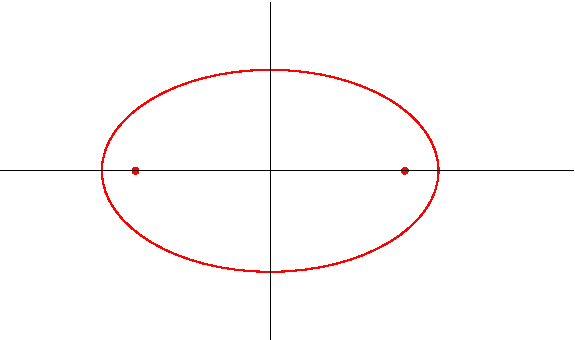
\includegraphics{Czuhobo_1.pdf}
 % Czuhobo_1.pdf: 3014770x7209072 pixel, 0dpi, infxinf cm, bb=
 \caption{Ellipse $\mathcal E_2$}
 \label{fig: Czuhobo_1}
\end{figure}
 
\end{enumerate}

\item 
\begin{enumerate}
 \item Un point $M$ de coordonnées $(x,y)$ est dans l'image par $Z$ de la demi-droite $D_\theta$ si et seulement si il existe un réel $r$ strictement positif tel que
\begin{align*}
 \dfrac{x}{\cos \theta}=r+\dfrac{1}{r} & & \dfrac{y}{\sin \theta}=r-\dfrac{1}{r}
\end{align*}
Il est clair que l'existence de ce réel $r$ entraine
\begin{displaymath}
 \left\lbrace 
\begin{aligned}
 \left( \dfrac{x}{\cos \theta}\right)^2 - \left( \dfrac{y}{\sin \theta}\right)^2 =& 4 \\
  \dfrac{x}{\cos \theta} >& 0
\end{aligned}
\right. 
\end{displaymath}
Pourtant, la condition $\frac{x}{\cos \theta} > 0$ n'est pas très bien choisie. Elle ne caractérise pas l'existence d'un $r>0$ tel que $\frac{x}{\cos \theta}=r+\frac{1}{r}$.\newline
D'après la question 1.b., la bonne condition est $\frac{x}{\cos \theta}\geq2$.\newline
Montrons que
\begin{displaymath}
 \left\lbrace 
\begin{aligned}
 \left( \dfrac{x}{2\cos \theta}\right)^2 - \left( \dfrac{y}{2\sin \theta}\right)^2 =& 1 \\
  \dfrac{x}{\cos \theta} \geq& 2
\end{aligned}
\right. 
\end{displaymath}
entraine l'existence d'un réel $r>0$ tel que 
\begin{align*}
 \dfrac{x}{\cos \theta}=r+\dfrac{1}{r} & & \dfrac{y}{\sin \theta}=r-\dfrac{1}{r}
\end{align*}
D'après la question 1.b., $\frac{x}{\cos \theta}\geq2$ entraine l'existence d'un $r>0$ tel que $\frac{x}{\cos \theta}=r+\frac{1}{r}$. On a vu qu'en fait il existe deux réels $r$ inverses l'un de l'autre. En remplaçant dans l'autre équation, on obtient
\begin{displaymath}
 \left( \dfrac{y}{\sin \theta}\right)^2 = 
\left( \dfrac{x}{\cos \theta}\right)^2 -4 =
r^2 + \dfrac{1}{r^2}-2=\left(r -\dfrac{1}{r} \right)^2 
\end{displaymath}
Si on remplace $r$ par son inverse, $r -\frac{1}{r}$ est remplacé par son opposé. Il existe donc un réel $r$ tel que l'on ait à la fois $\frac{x}{\cos \theta}=r+\frac{1}{r}$ et $\frac{y}{\sin \theta}=r-\frac{1}{r}$.\newline
Finalement, l'équation cartésienne de $\mathcal H_\theta$ est bien
\begin{displaymath}
 \left\lbrace 
\begin{aligned}
 \left( \dfrac{x}{2\cos \theta}\right)^2 - \left( \dfrac{y}{2\sin \theta}\right)^2 =& 1 \\
  \dfrac{x}{\cos \theta} \geq& 2
\end{aligned}
\right. 
\end{displaymath}

 \item La forme réduite d'une équation d'hyberbole apparait.\newline
La courbe $\mathcal H_\theta$ est donc une branche d'hyperbole contenue dans le demi-plan $\frac{x}{\cos \theta}\geq 2$. Le centre est $O$, l'axe focal $Ox$, la distance centre-foyer est 
\begin{displaymath}
 \sqrt{(2\cos \theta)^2 + (2\sin \theta)^2}=2
\end{displaymath}
, les foyers sont les points de coordonnées $(-2,0)$ et $(2,0)$, l'excentricité est $e=\frac{c}{a}=\frac{1}{\cos \theta}$.\newline
Les asymptotes sont les droites d'équation
\begin{align*}
 \dfrac{x}{2\cos \theta}-\dfrac{y}{2\sin \theta} =0
 & \text{ et } &
 \dfrac{x}{2\cos \theta}+\dfrac{y}{2\sin \theta} =0
\end{align*}
Leurs vecteurs directeurs sont $\overrightarrow{e_\theta}$ et $\overrightarrow{e_{-\theta}}$.
 \item L'équation cartésienne de $\mathcal{H}_{\frac{\pi}{3}}$ est
\begin{displaymath}
 x^2 - \dfrac{y^2}{3}=1 
\end{displaymath}
avec $x\geq 1$.
\begin{figure}[ht]
 \centering
\input{Czuhobo_2.pdf_t}
\caption{Branche d'hyperbole $\mathcal H_{\dfrac{\pi}{3}}$}
 \label{fig: Czuhobo_2}
\end{figure}
\end{enumerate}

\item D'après la question 1.b., l'image de $\mathcal D_0$ est la demi-droite $[2,+\infty[$.\newline
En multipliant par $-1$, il est clair que l'image de $\mathcal D_\pi$ est $]-\infty,-2].$\newline
Pour tout $t>0$,
\begin{displaymath}
 it + \dfrac{1}{it}= i \left( t-\dfrac{1}{t}\right) 
\end{displaymath}
De plus $t-\frac{1}{t}$ décrit $\R$ tout entier comme le montre l'étude des limites en $0_+$ et en $+\infty$. On en déduit que l'image de $\mathcal D_{\frac{\pi}{2}}$ et de $\mathcal D_{-\frac{\pi}{2}}$ est la droite $i\R$. 
\end{enumerate}

\subsection*{II. Coniques de Hooke}
\begin{enumerate}
 \item L'ensemble des solutions de l'équation différentielle $(1)$ est constitué par les fonctions
\begin{displaymath}
 z \rightarrow Ae^{k t} + be^{-kt}
\end{displaymath}
avec $A$ et $B$ complexes.
\item \begin{enumerate}
 \item Avec les notations de l'énoncé :
\begin{align*}
 A=|A|e^{i\alpha} & & B=|B|e^{i\beta} & & AB=|AB|e^{i(\alpha +\beta)}
\end{align*}
On en déduit:
\begin{displaymath}
 g=AB \Leftrightarrow g\in \left\lbrace \sqrt{|AB|}e^{i\frac{\alpha+\beta}{2}}, -\sqrt{|AB|}e^{i\frac{\alpha+\beta}{2}}\right\rbrace 
\end{displaymath}

\item Avec les définitions de l'énoncé :
\begin{displaymath}
 \left(\dfrac{A}{g} \right)^2=\dfrac{A}{B}=\dfrac{|A|}{|B|}e^{i(\alpha - \beta)} 
\end{displaymath}
donc
\begin{displaymath}
 \left(\dfrac{A}{g} \right)^2 \in \R \Leftrightarrow \dfrac{A}{B}\in \R
\Leftrightarrow \alpha - \beta \equiv 0 \mod \pi
\Leftrightarrow \alpha \equiv \beta \mod \pi
\end{displaymath}
Comme de plus $\frac{A}{B}=\frac{A\overline{B}}{|B|^2}$, on a aussi 
\begin{displaymath}
 \dfrac{A}{B}\in \R \Leftrightarrow A\overline{B} \in \R
\end{displaymath}
De même :
\begin{displaymath}
 \left \vert \dfrac{A}{g}\right\vert=1 \Leftrightarrow
\left \vert \dfrac{A}{g}\right\vert ^2 =1 \Leftrightarrow
\left \vert \dfrac{A}{B}\right\vert =1 \Leftrightarrow |A|=|B|
\end{displaymath}

\item Avec les notations de l'énoncé,
\begin{displaymath}
 S\circ Z(\dfrac{A}{g}e^{ikt})=
g\left( \dfrac{A}{g}e^{ikt}+\dfrac{g}{A}e^{-ikt}\right)=
Ae^{ikt} + Be^{-ikt} 
\end{displaymath}
\end{enumerate}

\item Les résultats de la question II.2 et de la partie I montrent que la trajectoire d'une solution de l'équation différentielle $(1)$ considérée comme une courbe paramétrée sont en général des coniques.\newline
En effet, une solution quelconque est de la forme
\begin{displaymath}
 z(t)=Ae^{kt}+Be^{-kt}= S\circ Z\left( \dfrac{A}{g}e^{kt}\right)\text{ avec }
 \dfrac{A}{g}e^{kt}=\sqrt{\left\vert \dfrac{A}{B}\right\vert}e^{i\frac{\alpha -\beta}{2}}e^{kt}
\end{displaymath}
La trajectoire de $z$ est donc l'image par les transformations $Z$ puis $S$ (qui est une similitude) de la trajectoire de
\begin{displaymath}
 t \rightarrow \dfrac{A}{g}e^{kt}
\end{displaymath}
Lorsque $K>0$, $k$ est réel, $\dfrac{A}{g}e^{kt}$ décrit la demi-droite $\mathcal D_{\frac{\alpha -\beta}{2}}$.\newline
Lorsque $K<0$, $k$ est imaginaire pur, $\dfrac{A}{g}e^{kt}$ décrit le cercle $\mathcal C_{\sqrt{\left\vert \frac{A}{B}\right\vert}}$.\newline
De plus,
\begin{align*}
 \dfrac{\alpha - \beta}{2}\equiv 0 \mod\dfrac{\pi}{2} \Leftrightarrow&
\alpha \equiv \beta \mod \pi \Leftrightarrow A\overline{B}\in \R \\
\sqrt{\left\vert \frac{A}{B}\right\vert}=1 \Leftrightarrow& |A|=|B|
\end{align*}
On en déduit les résultats suivants.

\begin{itemize}

 \item Pour $K>0$ et $A\overline{B}\not\in \R$. La trajectoire est une branche d'hyperbole
\begin{displaymath}
 S\circ Z\left( \mathcal D_{\frac{\alpha -\beta}{2}}\right)=S\left( \mathcal H_{\frac{\alpha -\beta}{2}}\right)  
\end{displaymath}
Les foyers sont les points d'affixe $-2g$ et $2g$. Les vecteurs directeurs des asymptotes ont pour affixe
\begin{align*}
 ge^{i\frac{\alpha -\beta}{2}}=\sqrt{|AB|}e^{i\alpha} & &
 ge^{-i\frac{\alpha -\beta}{2}}=\sqrt{|AB|}e^{i\beta}
\end{align*}
L'axe focal est la droite $(Og)$ bissectrice intérieure de $(OA),(OB)$. La distance centre-sommets est
\begin{displaymath}
 |g|\frac{1}{2\cos\frac{\alpha -\beta}{2}}=\dfrac{\sqrt{|AB|}}{2\cos\frac{\alpha - \beta}{2}}
\end{displaymath}

\item Pour $K>0$ et $A\overline{B}\in \R$, le carré du nombre complexe $\frac{A}{g}$ est réel. Par conséquent $\frac{A}{g}$ décrit une des quatre demi-droites $\mathcal D_0$, $\mathcal D_\frac{\pi}{2}$, $\mathcal D_\pi$, $\mathcal D_{-\frac{\pi}{2}}$. La trajectoire est soit une demi-droite soit une droite image par la similitude $S$ de $[2+\infty[$ ou $]-\infty,-2]$ ou de $i\R$. Il est à noter que lorsque la trajectoire est une demi-droite, celle-ci est parcourue deux fois : de l'infini vers le sommet puis du sommet vers l'infini.

\item Pour $K<0$ et $|A|\neq|B|$. La trajectoire de $z$ est une ellipse\footnote{En France ces ellipses sont dites de Lissajoux}.
\begin{displaymath}
 S\circ Z\left( \mathcal C_{\sqrt{\left\vert \frac{A}{B}\right\vert}}\right)
=S\left( \mathcal E_{\sqrt{\left\vert \frac{A}{B}\right\vert}}\right)  
\end{displaymath}
Les foyers sont les points d'affixe $-2g$ et $2g$. L'axe focal est la droite $(Og)$ bissectrice intérieure de $(OA),(OB)$. La distance centre-sommets (demi grand-axe) est
\begin{displaymath}
 \dfrac{|g|}{\sqrt{\frac{|A|}{|B|}}+\sqrt{\frac{|B|}{|A|}}}
= \dfrac{\sqrt{|AB|}}{\sqrt{\frac{|A|}{|B|}}+\sqrt{\frac{|B|}{|A|}}}
= \dfrac{|A||B|}{|A|+|B|}
\end{displaymath}
(en multipliant par $\sqrt{|AB|}$)

\item Pour $K<0$ et $|A|=|B|$, comme $k$ est imaginaire pur, le complexes $\frac{A}{g}e^{kt}$ est de la forme $e^{i\theta}$ et décrit un cercle de centre l'origine et de rayon 1. Or
\begin{displaymath}
 e^{i\theta}+\dfrac{1}{e^{i\theta}}=2\cos \theta
\end{displaymath}
donc la trajectoire est un segment image par la similitude $S$ de $[-2,2]$.
\end{itemize}


\item \begin{enumerate}
 \item Les conditions initiales conduisent aux équations
\begin{displaymath}
 \left\lbrace 
\begin{aligned}
 A+B =& z_0 \\
 kA - kB =& z'_0
\end{aligned}
\right. 
\Leftrightarrow 
\left\lbrace 
\begin{aligned}
 A =& \dfrac{1}{2}\left( z_0 + \dfrac{1}{k}z'_0\right)\\ 
 B =& \dfrac{1}{2}\left( z_0 - \dfrac{1}{k}z'_0\right)
\end{aligned}
\right. 
\end{displaymath}

 \item En utilisant les résultats de la question précédente, on obtient
\begin{displaymath}
 AB = \dfrac{1}{4}\left( {z_0}^2 - \dfrac{1}{K}{z'_0}^2\right) 
\end{displaymath}
et
\begin{multline*}
 A\overline{B} = \dfrac{1}{4}\left( z_0 + \dfrac{1}{k}z'_0\right)\left( \overline{z_0} - \dfrac{1}{\overline{k}}\overline{z'_0}\right)\\
= \dfrac{1}{4}\left( |z_0|^2 - \dfrac{|z'_0|^2}{|k|^2} 
+ \dfrac{z'_0 \overline{z_0}}{k} - \dfrac{z_0 \overline {z'_0}}{\overline{k}} \right)\\
= \dfrac{1}{4}\left( |z_0|^2 - \dfrac{|z'_0|^2}{|K|} +2i \Im\dfrac{z'_0 \overline{z_0}}{k} \right) 
\end{multline*}

 \item Pour $K<0$, le nombre $k$ est imaginaire pur. En comparant les carrés des expressions trouvées en $a$, on obtient 
\begin{displaymath}
 |A|=|B| \Leftrightarrow \Re\left( z_0\dfrac{\overline{z'_0}}{\overline{k}}\right)=0 
\Leftrightarrow z_0z'_0\in \R 
\end{displaymath}
On peut interpréter physiquement en considérant un point mobile \emph{attiré élastiquement} par un point fixé. Les trajectoires sont en général des ellipses (dites de Lissajoux). Dans le cas particulier où à un instant donné la vitesse est portée par la droite passant par le point et le centre, la trajectoire est un segment. 

 \item Dans le cas où $K>0$, le nombre $k$ est réel et
\begin{displaymath}
A\overline{B}\in \R \Leftrightarrow \Im\dfrac{z'_0 \overline{z_0}}{k}
\Leftrightarrow z_0\overline{z'_0}\in \R 
\end{displaymath}
Cette fois, le point mobile est \emph{repoussé élastiquement} par un point fixé. Les trajectoires sont des hyperboles sauf si à un instant donné la vitesse est portée par la droite contenant le centre et le point. Dans ce cas la trajectoire est une demi-droite ou une droite.
\end{enumerate}

\end{enumerate}


\subsection*{III. Transformation de Bohlin}
\begin{enumerate}
 \item \begin{enumerate}
\item Avec les propriétés usuelles des nombres complexes, il est bien clair que
\begin{align*}
 B(\mathcal{C} _r)= \mathcal C _{r^2} & & B(\mathcal D _\theta) = \mathcal D _{2\theta }
\end{align*}

\item L'affixe d'un point situé sur une droite d'équation $y=c$ est $z=t+ic$. L'affixe de son image par $B$ est
\begin{displaymath}
 z^2 = t^2-c^2 +2itc
\end{displaymath}
La partie réelle $x$ et la partie imaginaire $y$ vérifient donc 
\begin{displaymath}
 x= \left( \dfrac{y}{2c}\right)^2 - c^2 
\end{displaymath}
L'image par $B$ d'une droite d'équation $y=c$ est donc une parabole notée $\mathcal P_c$.\newline
Une droite $\Delta$ quelconque ne passant pas par l'origine est l'image d'une droite d'équation $y=c$ par une certaine similitude $s$ dont le point fixe est l'origine. Pour une telle similitude, $B\circ s = s^2 \circ B$. On en déduit que 
\begin{displaymath}
 B(\delta) = r^2(\mathcal p_c)
\end{displaymath}
Cette image est donc encore une parabole.
\end{enumerate}

 \item Il s'agit d'un calcul élémentaire :
\begin{displaymath}
 B\circ Z(z)=\left(z+\dfrac{1}{z} \right)^2
=(z^2 + \dfrac{1}{z^2})+2
=T\circ Z \circ B(z) 
\end{displaymath}

 \item D'après la partie I, 
\begin{displaymath}
 \mathcal E_r = Z(\mathcal C_r) \Rightarrow
B(\mathcal E_r) = B\circ Z (\mathcal C_r)= T\circ Z \circ B(\mathcal C_r)
=T\circ Z (\mathcal C_{r^2})= T(\mathcal E_{r^2})
\end{displaymath}
On en déduit que $B(\mathcal E_r)$ est encore une ellipse. De même, $B(\mathcal H_r)$ est encore une hyperbole 
\item
\end{enumerate}
